
\documentclass[11pt]{article}

\usepackage[utf8]{inputenc} % Required for inputting international characters
\usepackage[T1]{fontenc} % Output font encoding for international characters

\usepackage{mathpazo} % Palatino font
\usepackage{graphicx}
\usepackage{geometry}
\usepackage{float}
\usepackage{amsmath}
\usepackage{tabu}
\usepackage{array}
\usepackage{cellspace}
\usepackage[table]{xcolor}
\usepackage{multirow}
\usepackage{multicol}
\usepackage{placeins}
\usepackage{blindtext}
\usepackage{pdflscape}
\usepackage{hyperref}
\renewcommand{\baselinestretch}{1.25}
\geometry{margin=.75 in}

\begin{document}

%----------------------------------------------------------------------------------------
%	TITLE PAGE
%----------------------------------------------------------------------------------------

\begin{titlepage} % Suppresses displaying the page number on the title page and the subsequent page counts as page 1
	\newcommand{\HRule}{\rule{\linewidth}{0.5mm}} % Defines a new command for horizontal lines, change thickness here
	
	\center % Centre everything on the page
	
	%------------------------------------------------
	%	Headings
	%------------------------------------------------
	
	\textsc{\LARGE Portland State University
}\\[.25cm] % Main heading such as the name of your university/college
	
	\textsc{\Large Department of Electrical and Computer Engineering }\\[1cm] % Major heading such as course name

\includegraphics[width=0.2\textwidth]{psuLOGO.jpg}\\[1cm]	
	\textsc{\LARGE2019  ECE Capstone }\\[0.12cm] % Minor heading such as course title
	\textsc{\LARGE Team 21 }\\[0.12cm]	
		\textsc{\Large Faculty Advisor: Roy Kravitz, M.S. }\\[0.12cm]
		\textsc{\Large Sponsor: Jeremy Sarao, Sightline Applications }\\[1cm]
	
	%------------------------------------------------
	%	Title
	%------------------------------------------------
	
	\HRule\\[0.4cm]
	
	{\huge\bfseries UAV Landing Aid - Design Report}\\[0.4cm] % Title of your document
	
	\HRule\\[1.5cm]
	
	%------------------------------------------------
	%	Author(s)
	%------------------------------------------------
	

	{\Large\textit{Authors:}}\\
 	\Large\textsc{Kimball S. Davis}\\
	 \Large\textsc{Tai Pham} % Your name
	
	%------------------------------------------------
	%	Date
	%------------------------------------------------
	
	\vfill\vfill\vfill % Position the date 3/4 down the remaining page
	
	{\large\today} % Date, change the \today to a set date if you want to be precise
	
	%------------------------------------------------
	%	Logo
	%------------------------------------------------
	
	%\vfill\vfill
	%\includegraphics[width=0.2\textwidth]{PSULOGO}\\[1cm] % Include a department/university logo - this will require the graphicx package
	 
	%----------------------------------------------------------------------------------------
	
	\vfill % Push the date up 1/4 of the remaining page
	
\end{titlepage}

%----------------------------------------------------------------------------------------


\section*{Abstract}


 Integration of the SightLine Landing Aid for end users is problematic.  Often drone operators want to just “plug in” a component and fly their mission.  Installing software components is acceptable, but any requirement for programming is a barrier to entry or a complete show stopper.  Various cables, power, and other electrical connectivity issues are also difficult for vehicle integrator.  Rugged or at least robust mechanical enclosures, easy mounting, and environmental reliability are equally important.  Lastly, choice of optical system (camera) for the greatest range has cause adoption delays in that it has been a decision left to the integrator. Recognizing the needs from the end-users, SightLine wants to develop a plug and play precision landing aid for UAVs and expect that this new project will be highly valuable to a wide range of multi-copter integrator.
\\
 Our solution to the problem involves: I. Selecting, and building a consumer level quad-copter that will  be easily customizable for testing II. Designing a camera that will connect directly to the SightLine hardware, distribute power, and facilitate communication III. Research and development of documentation and software to meet plug and play expectations.
\\
 The selection, build, and testing of a custom quad-copter is a complicated task with many variables. GPS signal degradation made indoor flight tests impossible, and safe outdoor testing locations were hard to find. We did successfully build, and autonomously fly the Pixhawk4 controlled quad-copter using QGroundControl mission planning software. In the meantime, a camera for the SightLine hardware was designed utilizing an AR0134CS optical sensor. The camera board was also designed to provide power distribution, and facilitate communication between the Pixhawk 4 flight controller and the SightLine hardware.

*Insert SLA1500CAM Test Results summary Here*

Based on our project, the QGroundControl has demonstrated a great ability to control our quad-copter autonomously. The QGroundControl provides the ability to fully control all quad-copter parameters and as well as setting up a mission. We have successfully flied the drone autonomously using QGroundControl includes takeoff, land, fly the mission, and return to land. The precision landing feature on QGroundControl is not very promising. For the simple function like takeoff and landing, the position between takeoff and land was about 1 meter. For the flying to a destination and return, the difference in position was 2 meter. Additionally, before doing the flight test, we also use Mission Planner to simulate the flight and learn how to control the quad-copter's parameters.
   
*What are the limitations?
The limitation comes from both QGroundControl and SightLine hardware. Since SightLine hardware, or 1500-SLA-kit, is unable to talk with QGroundControl and as well as, we don't know if QGroundControl is capable of talking to SightLine hardware. There will be some works that SightLine need to be done with their hardware  so it will be able to talk with QGroundControl.  

*What are the Future implications of the project?*
The project is now divided into two parts. The first part is understand the Ground Control State software (QGroundControl) and hardware  such as Pixhawk 4, and SLA1500CAM. The second part will emphasize in software and communication development. SightLine and our team has determined to leave the second part of the project for the future capstone team. With our achievements on this project, we have a strong belief that the future team will be successful in this project and future function development.

\pagebreak

\tableofcontents

\pagebreak

\listoffigures

\pagebreak

\section{Project Overview}
\subsection{Background}
SightLine Applications has developed a precision visual landing algorithm that provides an excellent set of benefits:
\begin{itemize}
\item Works in degraded and denied GPS environments – Safety and reliability
\item	Reduces operator training and landing phase complexity.
\item	Provides detection functions for landing zone safety - detect people, animals, or objects from entering the landing zone
\item   Provides a rich set of telemetry for flight controllers.  30 Hz data with range, XY offsets, relative azimuth, etc.
\item	Supports landing on moving platforms - ground vehicles, marine.
\item	Is not impacted by bright sun or low light conditions.
\item	Can be used with Thermal (IR) cameras as well as visible (EO) cameras
\item	Effective range of operation (distance to target) only limited by the size of the landing pattern used
\end{itemize}

\subsection{Problem Definition}

Integration of the SightLine Landing Aid for end users is problematic for two main reasons: 

\begin{enumerate}
\item Connectivity issues with a wide range of cameras. 
\item Communication issues with a wide range of flight controller hardware and software.
\end{enumerate} 

Currently the end user selects a camera to be used with the SightLine processing hardware. A wide range of cameras must be supported, and custom AB boards must be designed for each one to interface with the SightLine hardware. Each of these AB boards can have cable, power, and electrical connectivity issues that are problematic for the end user.
There is also a wide range of flight controller hardware and software, each with a myriad of different communication protocols. Installing software components to facilitate this communication is fine for the end user, but if any programming needs to be done this is usually a complete show stopper. 

\subsection{Solution}

The proposed solution to these problems is to develop an all in one unit (SightLine Hardware w/Camera) with plug and play capabilities that can be directly connected to a consumer level flight controller. By doing so camera connectivity and selection problems are eliminated, and communication and software deployment are made much easier for the end user. We will build an off the shelf quad-copter with autonomous flight capabilities to test communication between current SightLine hardware, and our newly designed camera interface.

\subsection{Project Management}

The project is divided into three sections:
\begin{enumerate}
 \item Choosing and building an "off the shelf" quad-copter that uses a Pixhawk 4 flight controller that can be used for testing
 \item Designing a camera based on the On-Semi AR0134CS optical sensor that connects directly to the SightLine hardware, distributes power, and facilitates communication  between the flight controller and SightLine hardware
 \item Research and development of documentation and software installers to meet plug and play expectations using QGroundControl flight control and mission planning software
\end{enumerate}
*Insert Project Roles and Responsibilities here*

\subsubsection{Project Timeline}

\begin{figure}[h!bt]
\centering	
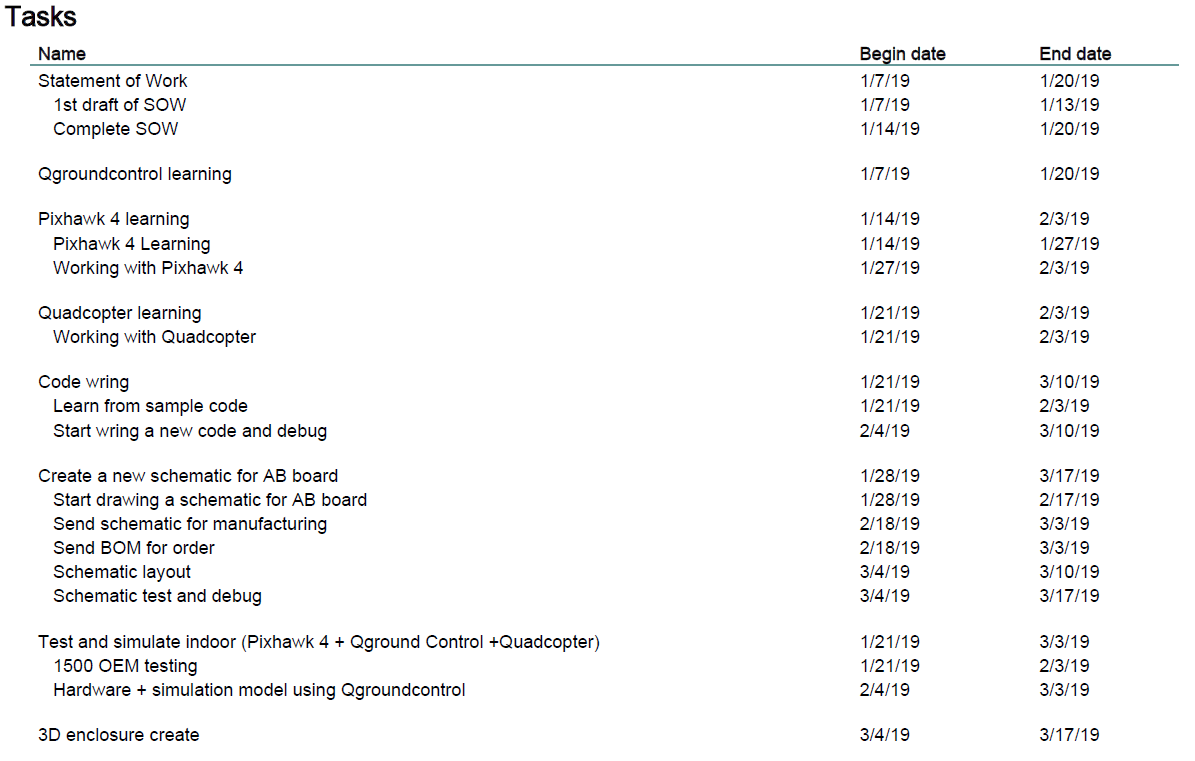
\includegraphics[width=7 in]{timeline1}
%\caption{\textit{Simple saturable reactor[1]}}	
\end{figure}

\begin{figure}[h!bt]
\centering	
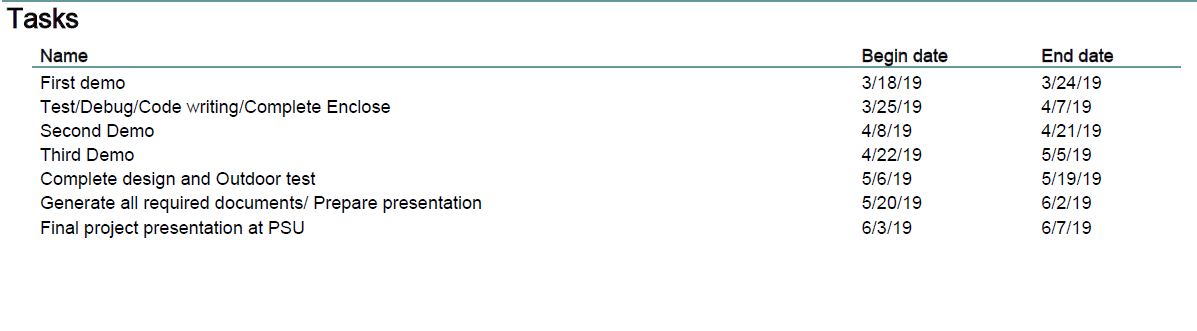
\includegraphics[width=7 in]{timeline2}
\caption{\textit{Project Timeline}}	
\end{figure} 
\break

Above is the project timeline which was created at the beginning of the Winter term. However, things have changed a lot during our capstone, and the timeline above is just for reference.


%    \begin{figure}[H]
%	\centering	
%	\includegraphics[width=3.5 in]{Simple_SatR}
%	\caption{\textit{Simple saturable reactor[1]}}	
%	\end{figure}

\section{Results(Technical Detail)}
\subsection{Quadcopter}

In this project, we used a DJI Flame F450 as the core for our custom quadcopter design. The parts and accessories are indicated in figure below. The total quadcopter's cost is \$989.29. In the end of the project, we have successfully optimized the automonous flight and control using Qgroundcontrol. Therefore, the radio transmitter and its receiver is no longer neccessary which brought the cost down to \$728.3 for the future experiment. \newline 
With the 4S battery, the quadcopter has 15 minutes flying time, and the maximum take-off weight is  around 800g. Based on our experiment, the custom quadcopter has demonstrated safe and stable flights, and can be fully controlled by Groundcontrol Station.  
\newpage
\begin{figure}[h!bt]
\centering	
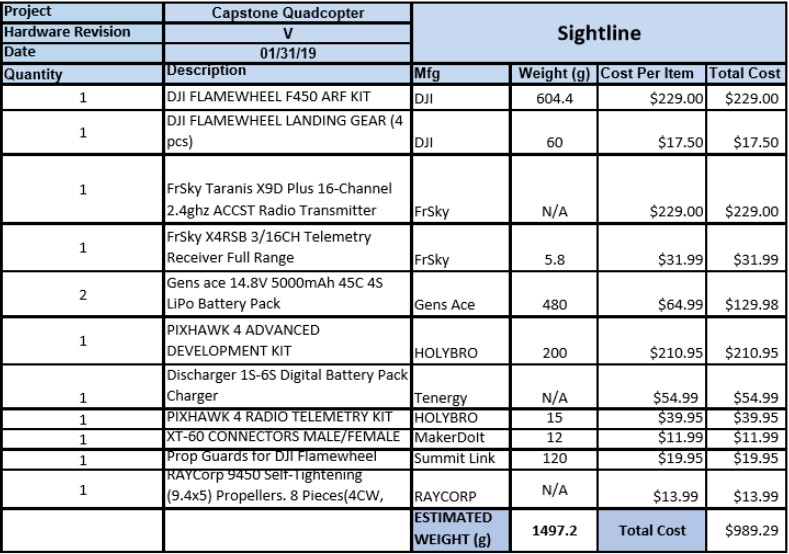
\includegraphics[width=7 in]{quadcopter_part}
\caption{\textit{Quadcopter's parts and accessories}}	
\end{figure} 

\begin{figure}[h!bt]
\centering	
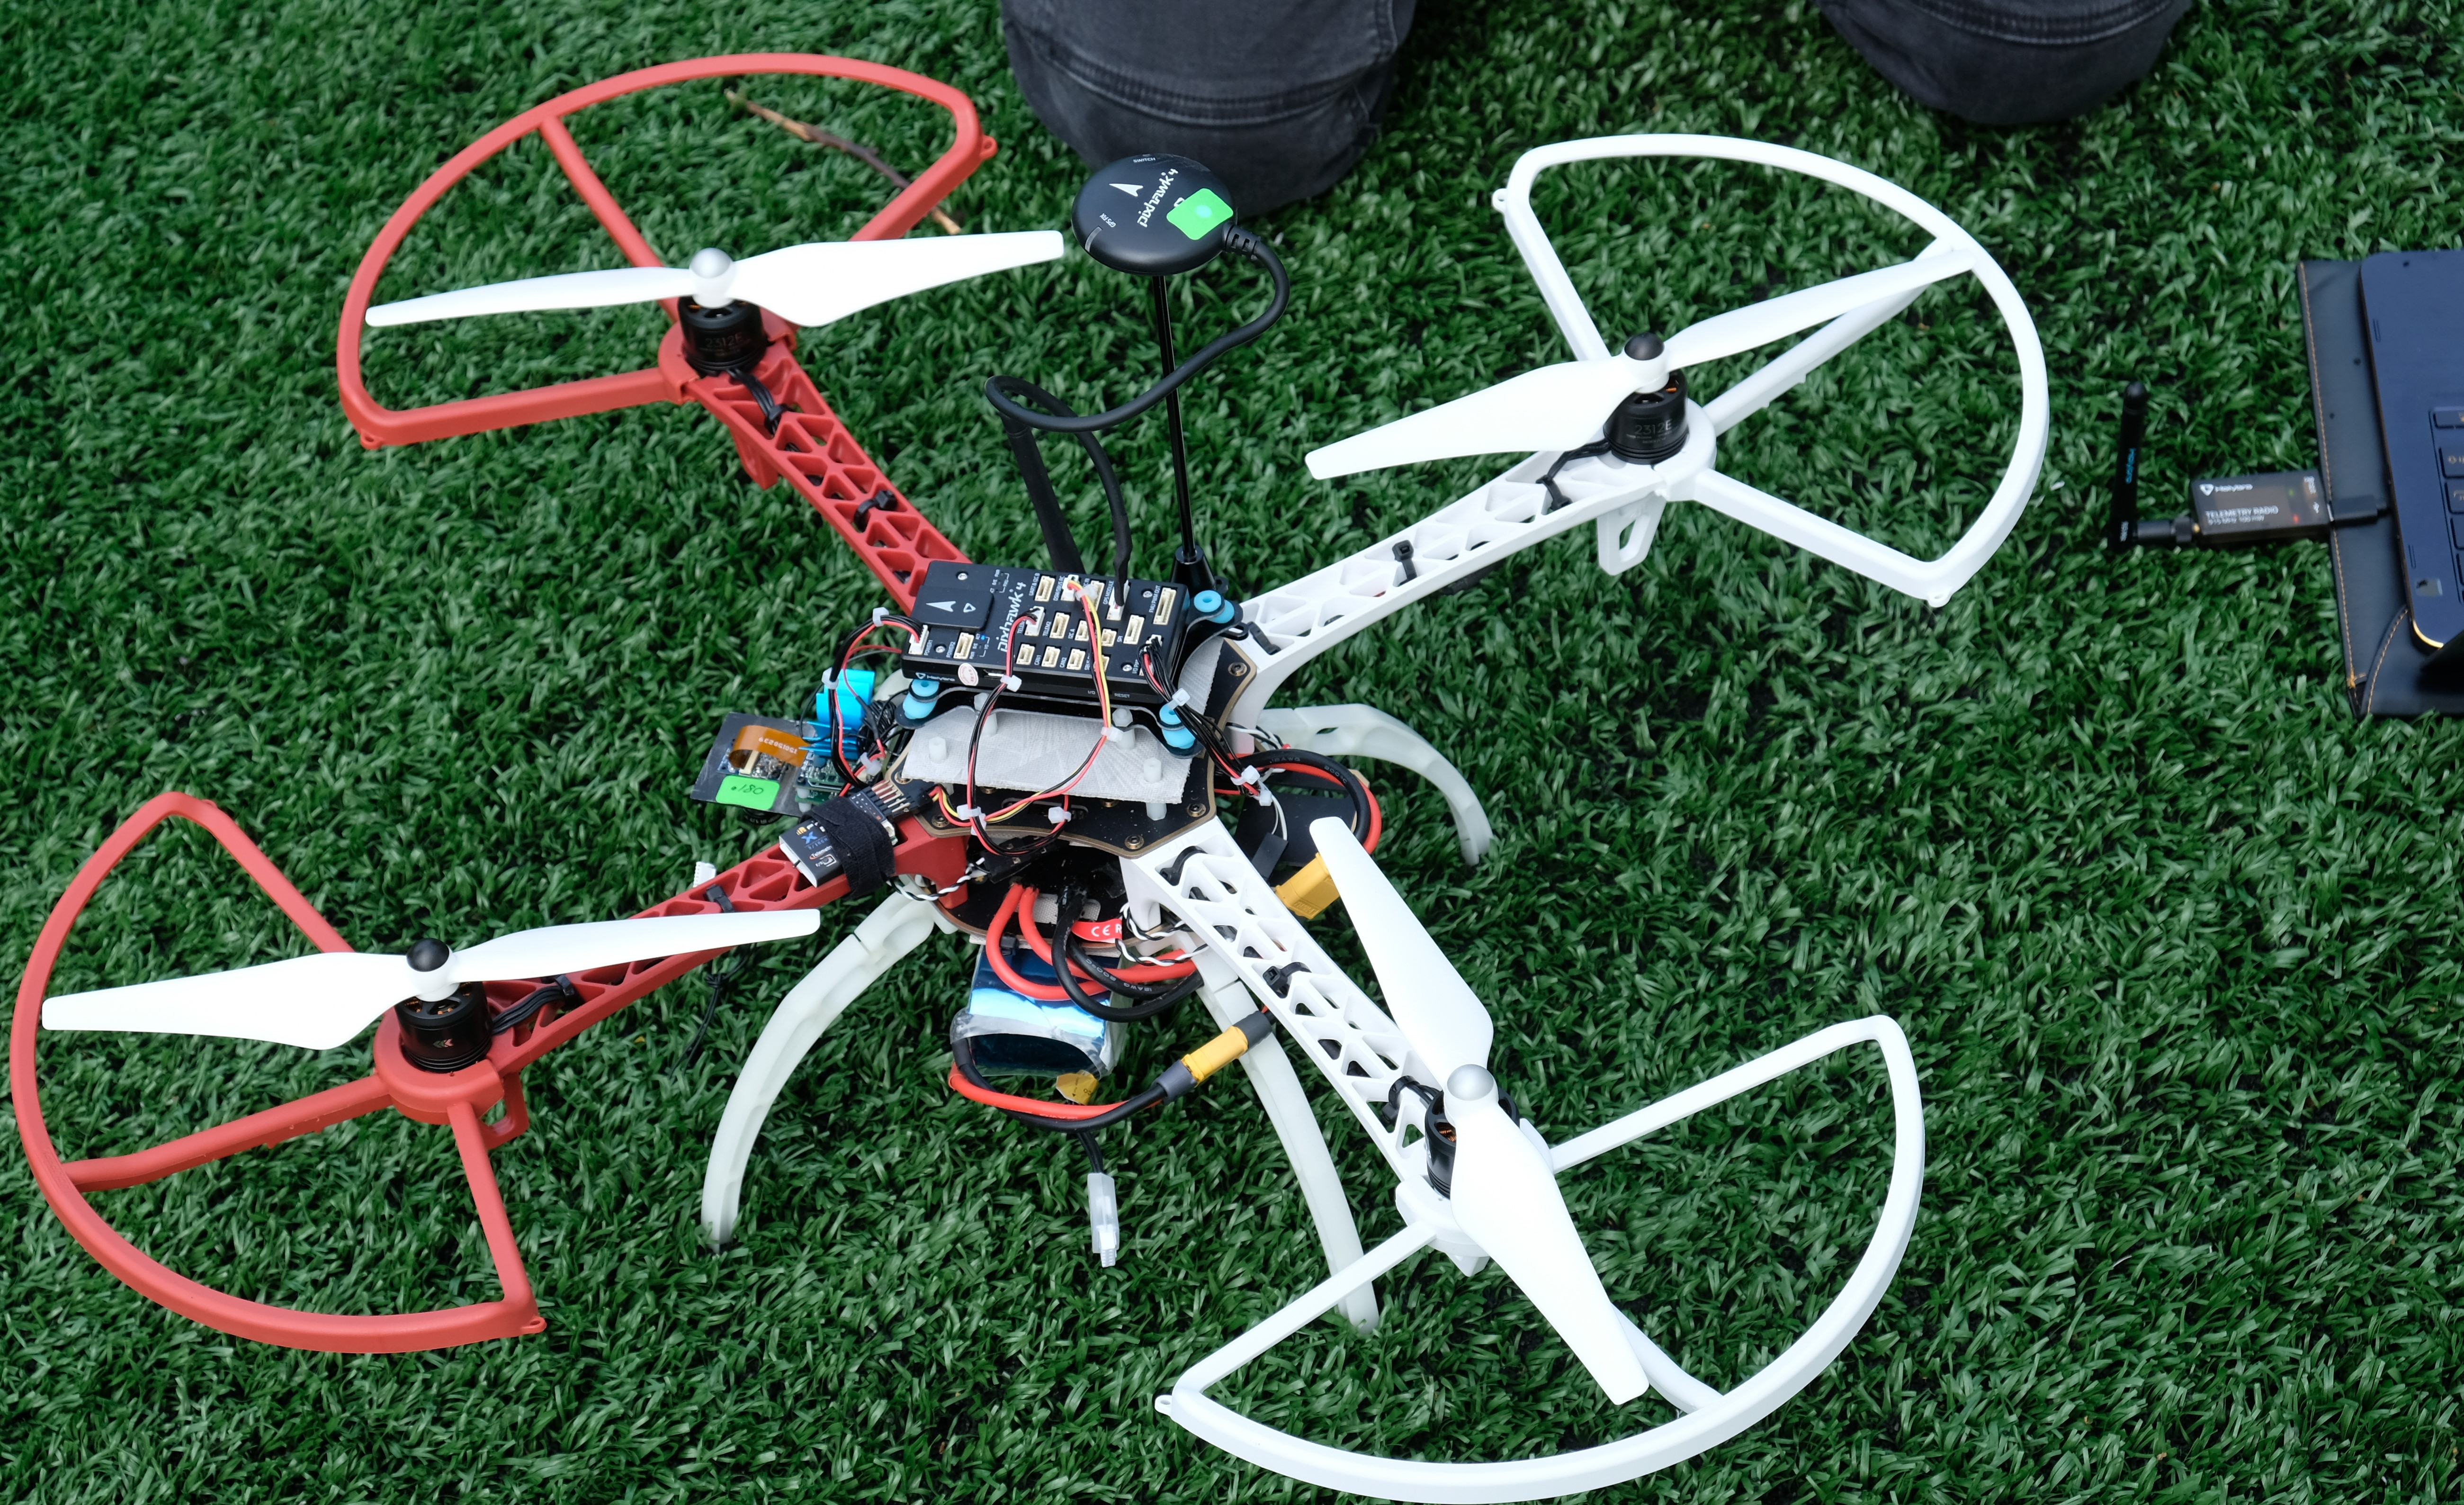
\includegraphics[width=4.5 in]{quad}
\caption{\textit{Custom Quadcopter}}	
\end{figure}

\subsection{Pixhawk 4}
Pixhawk 4 is a flight controller made by Holybro and PX4. Pixhawk 4 is one of the modest flight controllers and has worked stably with number of autopilot softwares such as Qgroundcontrol and Mission Planner. Pixhawk 4 is our best choice for this project because of following reasons:

\begin{itemize}

\item Light weight - only 15.8g
\item Multi options for communication protocol such as I$^2$C, CAN, and several SBUS.
\item Built-in GPS and provide the port for external GPS
\item Easy to setup with Qgroundcontrol
\item Provide plug-and-play ability     

\end{itemize}

\begin{figure}[h!bt]
\centering	
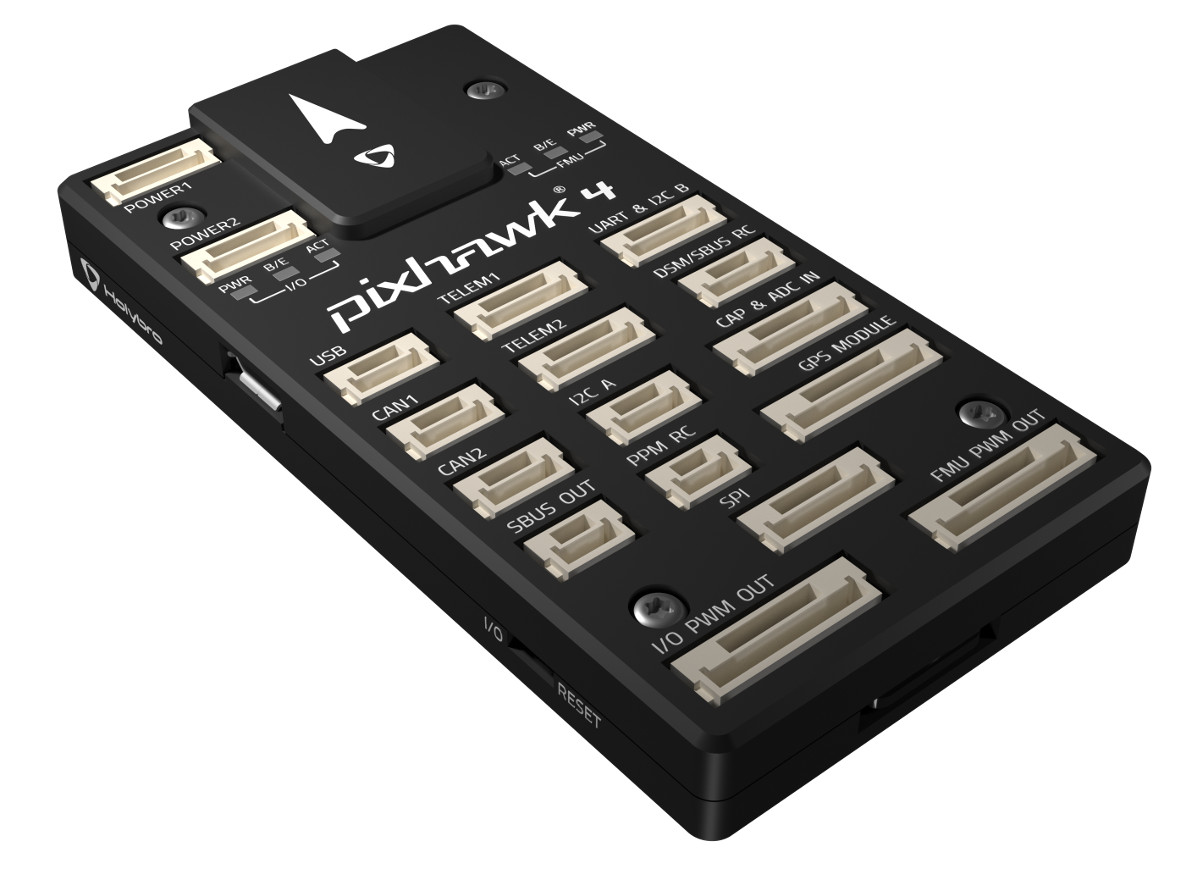
\includegraphics[width=4.5 in]{pixhawk4}
\caption{\textit{Pixhawk 4}}	
\end{figure}

\subsection{Hardware}

The 1x1.5” SLA1500CAM utilizes the On-Semi AR0134CS, a monochrome 1/3-inch 1.2 Mp CMOS digital sensor with a 74MHz output. It connects seamlessly with the SightLine SLA1500OEM image processing hardware via a 50-pin Hirose DF12 connector. With a 5V input the SLA1500CAM  converts and distributes the 3.3V, 2.8V, and 1.8V required for operation.



    \begin{figure}[H]
	\centering	
	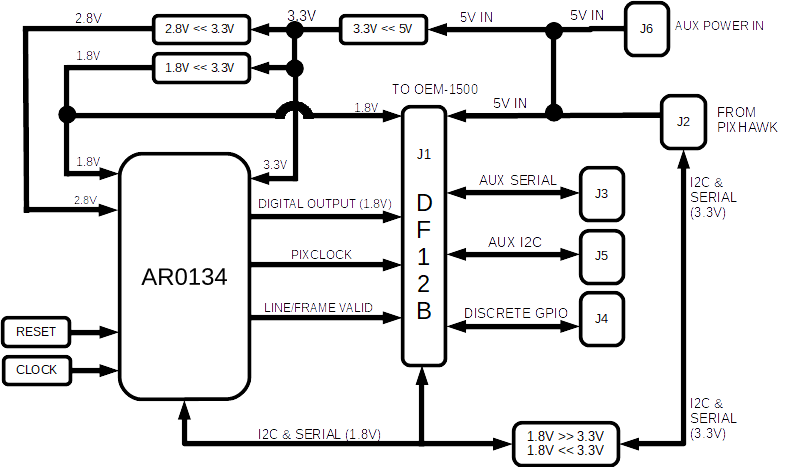
\includegraphics[width=6 in]{LEVEL1_DIAGRAM_SCHEM_V2}
	\caption{\textit{Level 1 block diagram of SLA1500CAM REV 8.0}}	
	\end{figure}

The SLA1500CAM also provides bi-directional level translation for serial and I2C communication between the SightLine hardware, the flight controller, and the optical sensor. There are five I/O ports using standard Molex and JST connectors: 

\begin{itemize}

\item Power and serial communication for the flight controller
\item Auxiliary I2C bus
\item Auxiliary serial communication
\item Auxiliary power in 

\end{itemize}



\subsection{Connector Summary}

    \begin{figure}[H]
	\centering	
	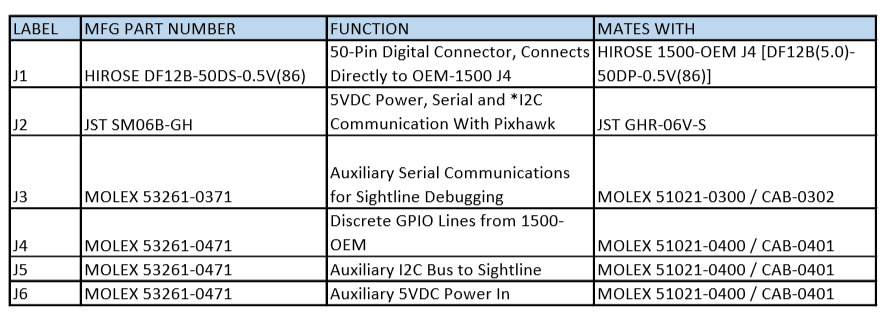
\includegraphics[width=7 in]{SLA1500CAM_CONN_V3}
	\caption{\textit{Connector summary for SLA1500CAM REV 8.0}}	
	\end{figure}

\subsubsection{Connector J1}

Digital camera, serial, power for SLA1500OEM
\\
This connector is designed to mate with the SLA1500OEM J4 connector. 

    \begin{figure}[H]
	\centering	
	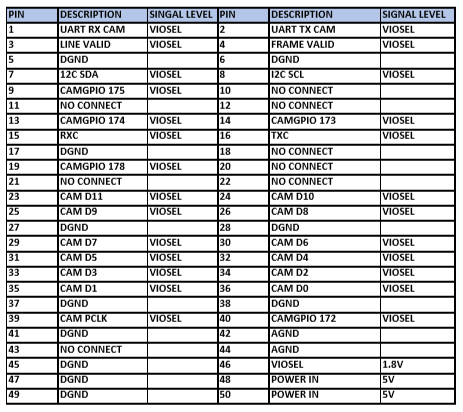
\includegraphics[width=6 in]{CONN_J1}
	\caption{\textit{Connector summary for J1}}	
	\end{figure}

 The GPIO connections for J1 are as follows:

\begin{itemize}

\item CAMGPIO 172 is connected to DNP Resistor R7 to AR0134 TRIGGER
\item CAMGPIO 173  is connected to DNP Resistor R8 to AR0134 FLASH
\item CAMGPIO 174  is connected to AR0134 RESET
\item CAMGPIO 175  is connected to AR0134 STANDBY
\item CAMGPIO 178 is connected to DNP resistor R26 to AR0134 OEBAR
\end{itemize}

AR0134 OEBAR is tied to ground with 0 OHM resistor R27.

\textbf{*R27  MUST BE REMOVED BEFORE R26 IS INSTALLED AND CAMGPIO 178 CAN BE USED.}



\begin{landscape}
   \begin{figure}[H]
	\centering	
	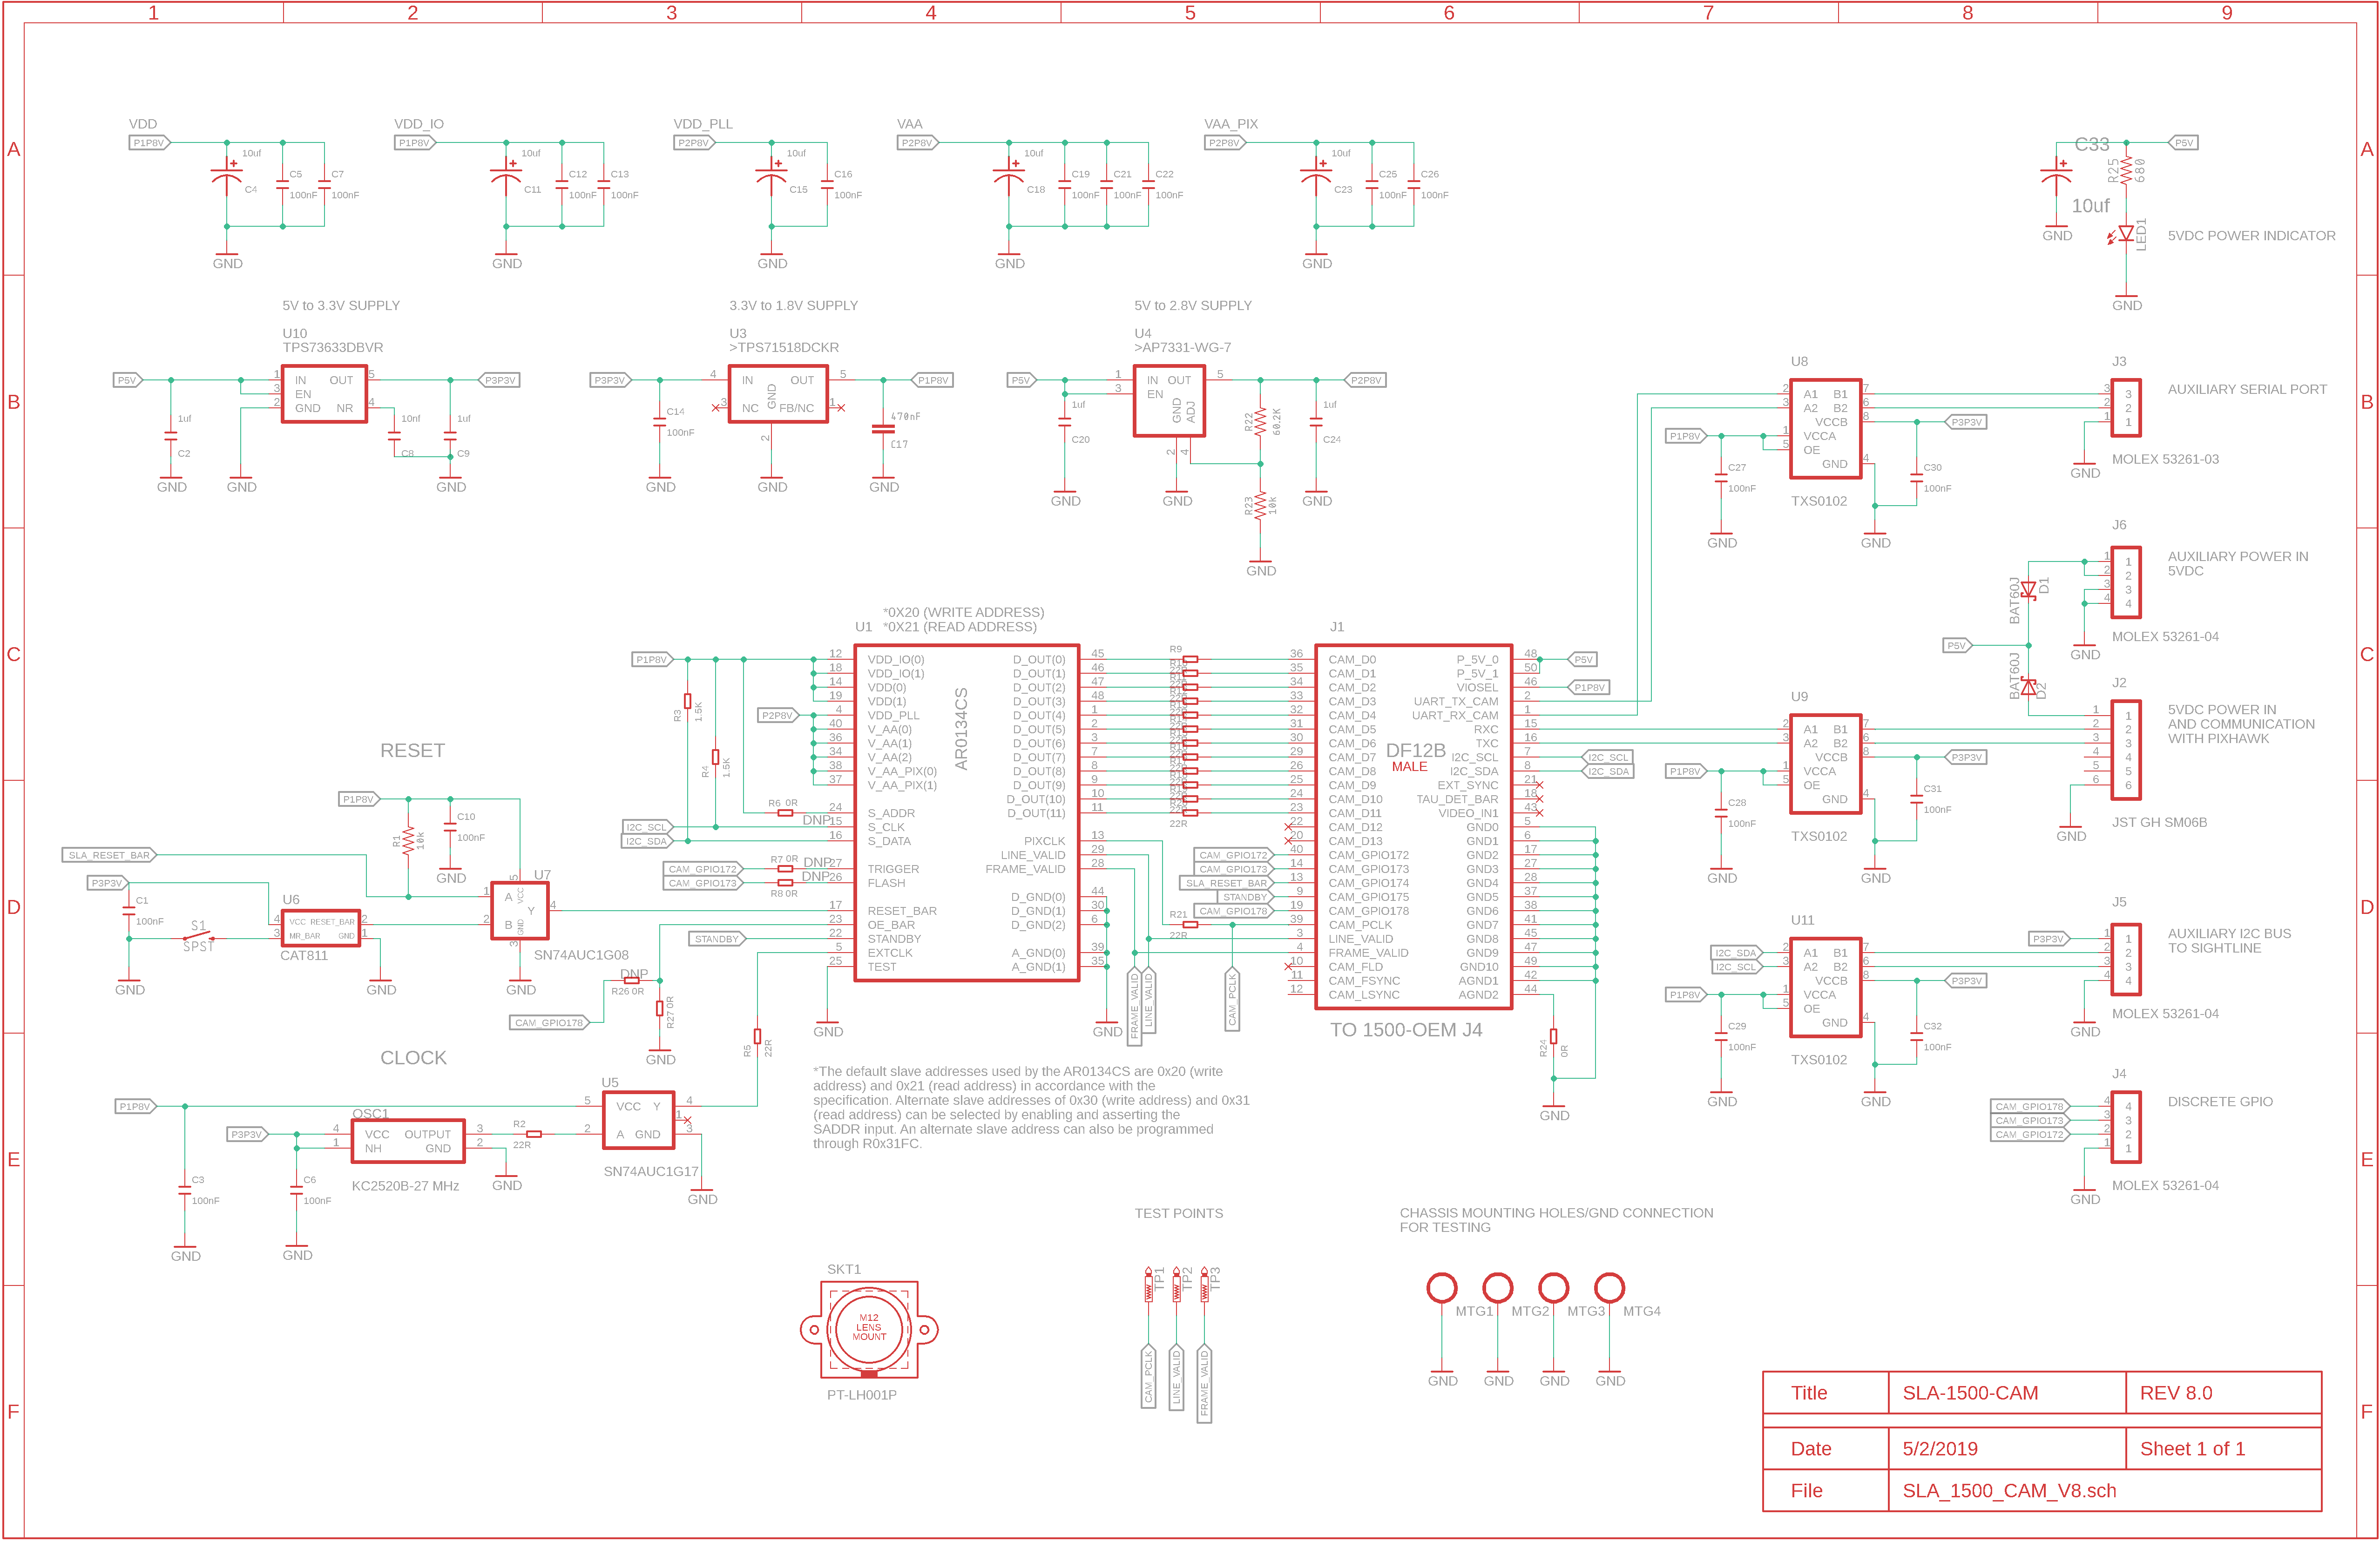
\includegraphics[width=9.5in]{SLA1500CAM_V8_sch}
	\caption{\textit{SLA 1500 CAM REV 8.0 Schematic}}	
	\end{figure}
\end{landscape}


    \begin{figure}[H]
	\centering	
	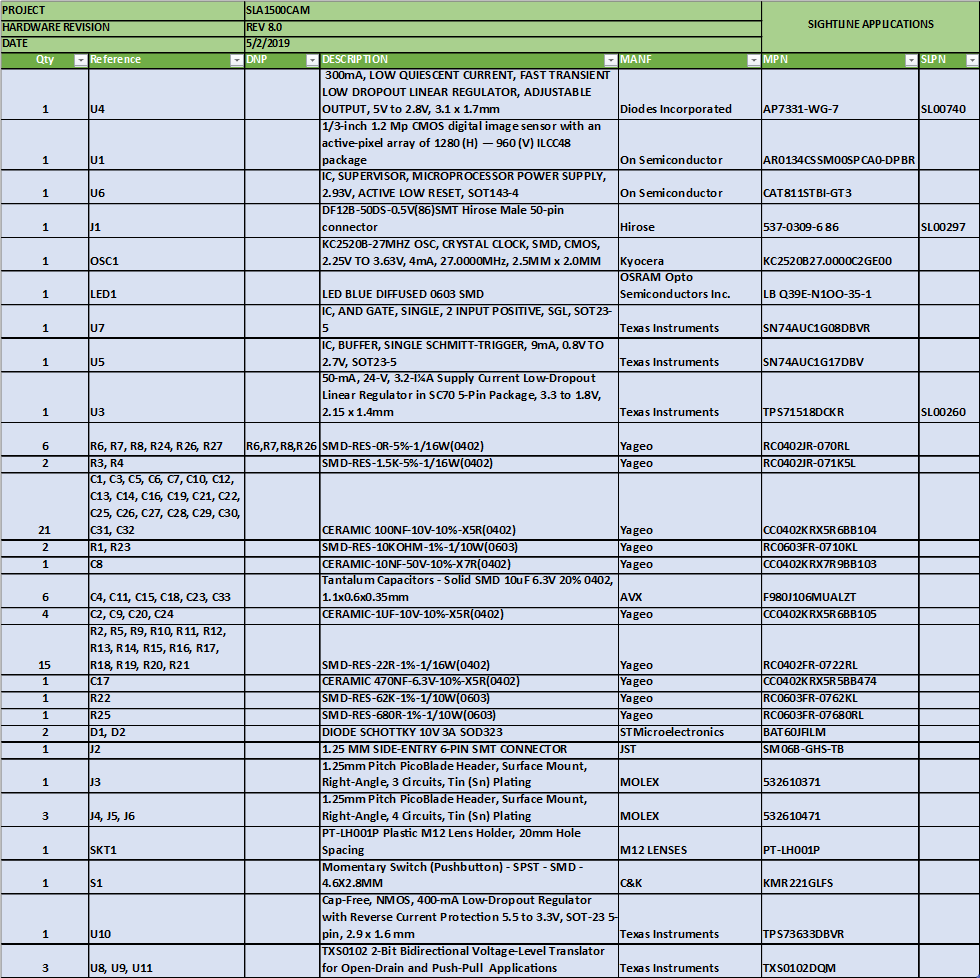
\includegraphics[width=7 in]{SLA1500CAM_BOM_V8}
	\caption{\textit{SLA1500CAM BOM REV 8.0}}	
	\end{figure}

The schematic and PCB were designed using EAGLE CAD 9.2.1. Many of the component footprints and devices were unavailable and were designed specifically for the project. This involved designing the device, footprint, schematic symbol, and linking material data to each device. The entire EAGLE library for the SLA1500CAM can be found in the GitHub repository.

\href{https://github.com/phamtaiece/Capstone-Sightline/tree/master/EAGLE\%20files/Library}{Eagle Library for SLA1500CAM}





\subsection{Software}

\subsubsection{Qgroundcontrol}
Qgroundcontrol is an open-source software which allows users/developers design and optimize their own unmanned aerial vehicle. The laptop that installs the Qgroundcontrol is called Ground Control Station (GCS). Qgroundcontrol allows users/ developers adjust and control every single parameter of the drone as well as set up a mission for the drone flying autonomously including take-off and precision landing. Qgroundcontrol is developed by PX4, and it's optimized to work best with Pixhawk family especially Pixhawk 4. By using a transmitter telemetry and a receiver telemetry, Qgroundcontrol can send the command to the Pixhawk 4 and then control the quadcopter wirelessly which provides a great opportunity to develop  plug-and-play ability for quadcopter and Sightline SLA-1500-CAM. \newline
Our project has proved that Qgroundcontrol can fully control and communicate with the quadcopter even when the quadcopter is up in the air.  

\begin{figure}[h!bt]
\centering
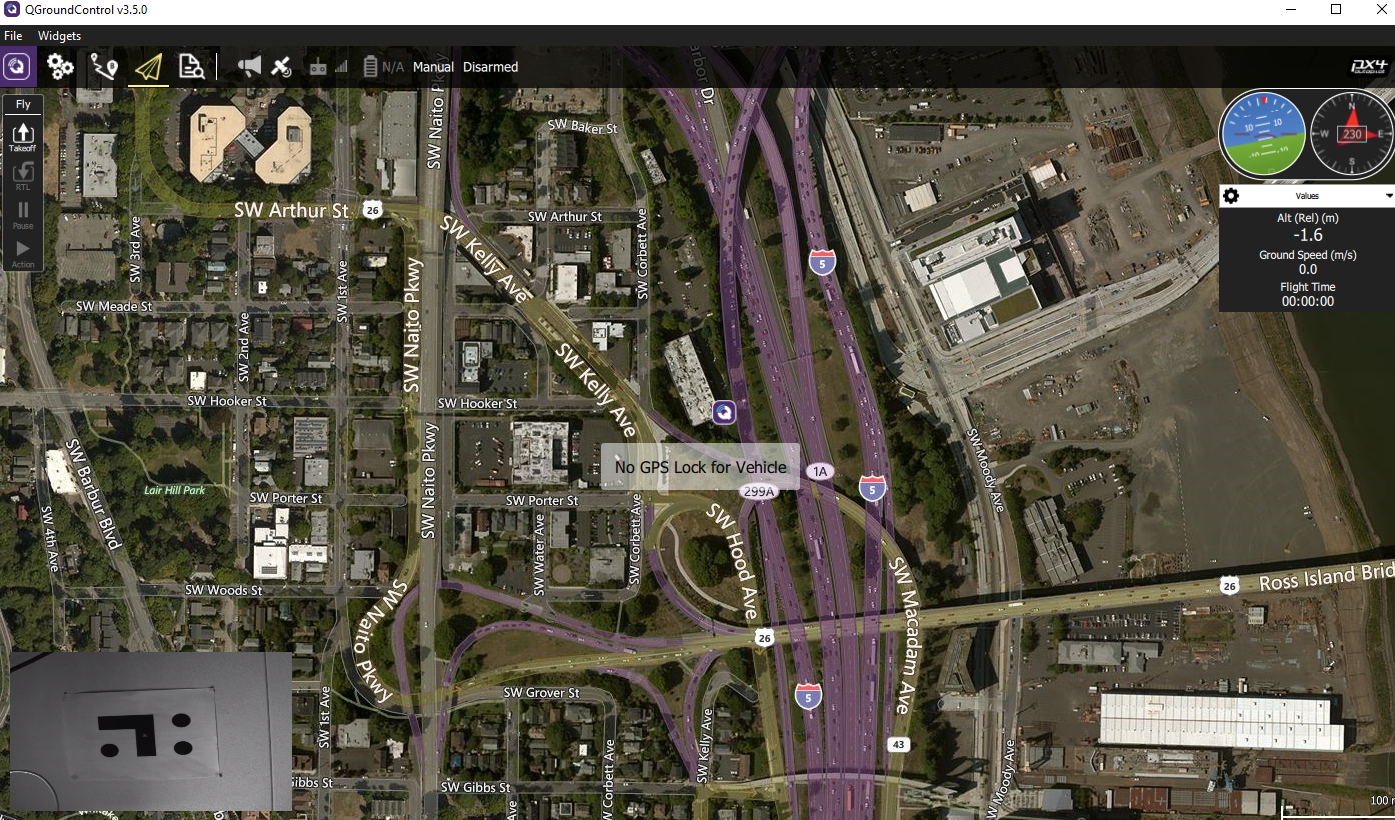
\includegraphics[width=4.5 in]{Qgroundcontrol}
\caption{\textit{Qgroundcontrol}}	
\end{figure}
\subsubsection{Mission Planner}
Alternatively, Mission Planner is a autopilot software which is developed by Ardupilot team. Similar to Qgroundcontrol, Mission Planner provides a good way to control the drone autonomously as well as adjust the drone's parameters. In this project, the Mission Planner is used to simulate the drone's behavior virtually by using Software In The Loop (SITL) technique. The SITL technique is extremely helpful in understanding the drone's behaviors and how to control the drone wirelessly without crashing an actual drone. The simulation provides varieties of tools and command that can change the speed of drone, speed and direction of wind, precision landing, and flight mode. \newline
\begin{figure}[h!bt]
\centering
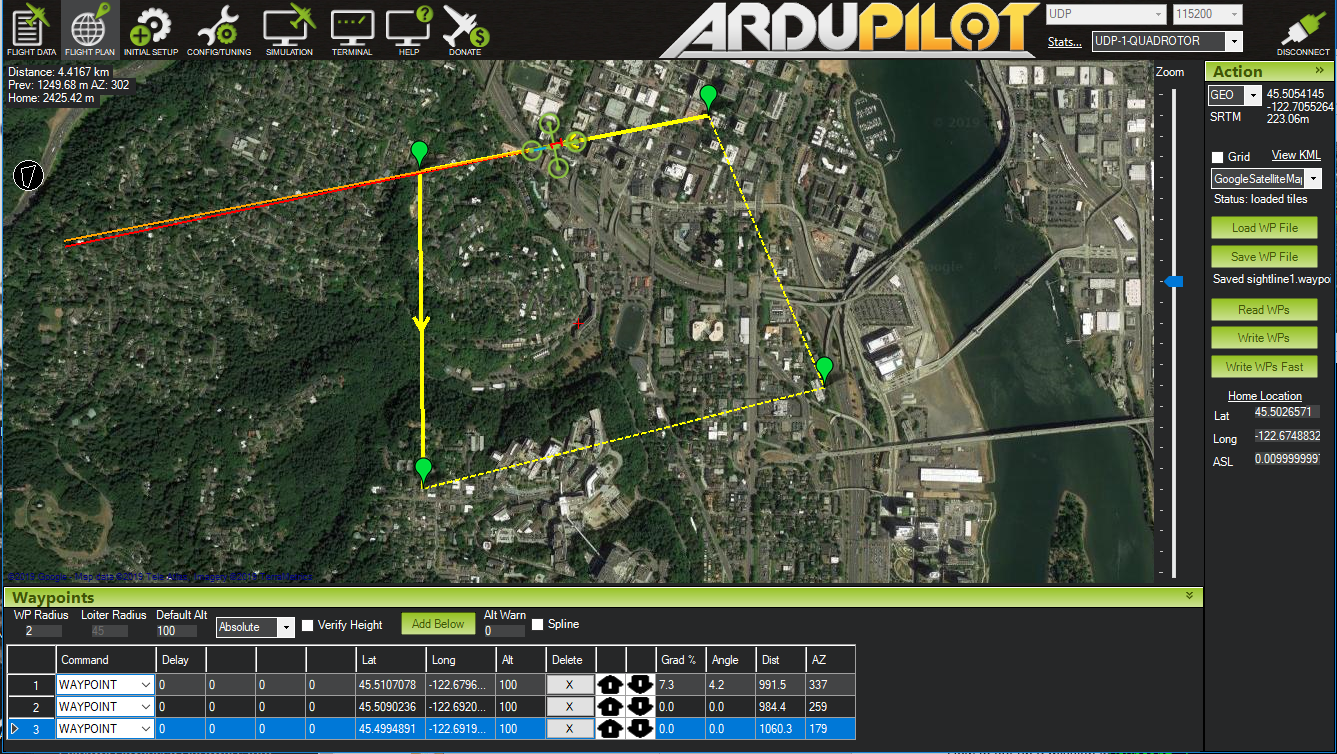
\includegraphics[width=4.5 in]{mission}
\caption{\textit{Setup a mission in Mission Planner}}	
\end{figure}
     

\section{Conclusion/What's Left to do}
Throughout the capstone project, we have gained a lot of experience which is not only academic experience but only real world experience, and how to deal with some problems in a team. On the project side, we have successfully developed the SLA-1500-CAM. However, due to manufacturing delay, we haven't had a chance to test the board yet. We have also gain insight into communication between Qgroundcontrol, Pixhawk4, and Sightline SLA-1500 kits. \\
We have successfully completed autonomous flight and landing with custom quadcopter with flight controller, Pixhawk4, and Qgroundcontrol. Importantly, we were able to record the video when the vehicle was up in the air by using SLA-1500 kits which promissingly provides the ability to develop plug-and-play feature in the future with SLA-1500-CAM, Qgroundcontrol and Pixhakw4. \\
However, The compability issues remain with Qgroundcontrol and Sightline hardware because Sightline SLA-1500 kits wasn't able to send the signal to Qgroundcontrol. Potentially, a new project will focus on software and communication between SLA-1500-CAM and Qgroundcontrol for a future team that is interested in drone communication protocols. With our achievements on this project, we believe that full integration of the SLA-1500-CAM with plug and play capabilities can be achieved.     

\pagebreak

\section{Appendix}
\subsection{I}
\subsection{II}
\subsection{II}
\subsection{IV}
\subsection{V}	

\pagebreak

\section{References}
\begin{enumerate}
\item Mali, P. (1960).\textit{ Magnetic Amplifiers}. New York, NY: John F. Rider.
\item Figure 1. Simple saturable reactor. Reprinted from \textit{Magnetic Amplifiers}(pg. 27), by Paul Mali, 1960, New York, NY, John F. Rider Publisher, Inc.
\item Figure 2. Full-wave self-saturating magnetic amplifier. Reprinted from \textit{Magnetic Amplifiers}(pg. 35), by Paul Mali, 1960, New York, NY, John F. Rider Publisher, Inc.
\end{enumerate}	
\end{document}
